
%(BEGIN_QUESTION)
% Copyright 2010, Tony R. Kuphaldt, released under the Creative Commons Attribution License (v 1.0)
% This means you may do almost anything with this work of mine, so long as you give me proper credit

This paint mixing system mixes (clear) base and (colored) pigment to achieve a desired coloring, according to the ratio setpoint:

$$\includegraphics[width=15.5cm]{i04510x01.eps}$$

Determine what will happen to the paint's color over time if the pigment flowmeter turbine seizes so that it does not turn even when there is adequate flow through the pipe.  Also, explain {\it why} the paint's color will be affected as you predict.

\underbar{file i04510}
%(END_QUESTION)





%(BEGIN_ANSWER)

The paint will become more and more colored over time, as the control system turns up the flow of pigment.  This will happen because the ratio control system sees no pigment flow anymore, and thus turns the pigment flow on fully to try to reach setpoint.

%(END_ANSWER)





%(BEGIN_NOTES)


%INDEX% Control, strategies: ratio

%(END_NOTES)


